% -%-%-%-%-%-%-%-%-%-%-%-%-%-%-%-%-%-%-%-%-%-%-%-%-%
% PIM380                                           %  
% 10/06/2013                                       %
% -%-%-%-%-%-%-%-%-%-%-%-%-%-%-%-%-%-%-%-%-%-%-%-%-%
\documentclass[compress,pdf,11pt,xcolor=dvipsnames]{beamer}

\usepackage[francais]{pim}

\title{Reconstruction 3D temps-réel HD de visages}                               
\usenavigationsymbolstemplate{}
\setbeamertemplate{footline}[] 
%\setbeamertemplate{ffootlineg}{}%remove navigation symbols
%\beamertemplatenavigationsymbolsempty 
%\setbeamertemplate 
%%% title page %%%
\subtitle{PIM380} 
\author[Tiago Siva, Vinicius Gardelli]{
  Tiago Chedraoui Silva \and
  Vinicius Dias Gardelli\\
}
\institute{Télécom Paristech}
\date{Juin 28, 2013}


\begin{document}

\begin{frame}
  \titlepage
\end{frame}

\begin{frame}{Plan}
  \tableofcontents
\end{frame}

\section{Introduction}

\begin{frame}{Les animations faciales}

        \begin{block}{Objectif}
          \begin{itemize}
          \item Capturer des performances expressives très
          détaillées
          \end{itemize}
        \end{block}

        \begin{alertblock}{Préocupation}
          \begin{itemize}
          \item Temps de configuration 
          \item Invasion au acteur 
          \end{itemize}
        \end{alertblock}

        \begin{exampleblock}{Situation}
          \begin{itemize}
          \item Convergenge aux captures passives
          \end{itemize}
        \end{exampleblock}

%  \begin{block}

%    \begin{columns}
%      \begin{column}{0.5\textwidth}
%        \begin{block}{Objectif}
%          Capturer des performances expressives très
%          détaillées
%        \end{block}
%      \end{column}
%      \begin{column}{0.5\textwidth}
%        \begin{alertblock}{Préocupation}
%        Temps de configuration \\
%        Invasive au acteur 
%        \end{alertblock}
%      \end{column}
%      \end{columns}
      
      
%      \begin{description}
%      \item [\color{orange}Objectif \hfill] Capturer des performances
%        expressives très détaillées \hfill 
%      \item [\color{red}{Préocupation}]Temps de configuration,
%        invasive au acteur 
%      \item [\color{blue}{Situation} \hfill] \hfill Plusieurs approches dans les
%        deux décennies
%      \end{description}
%    \end{block}
  \end{frame}

%\subsection{Le context}
\subsection{Etat de l'art}

\begin{frame}{Les méthodes de capture}
  
  \begin{columns}
    \begin{column}{0.5\textwidth}
      \pgfputat
          {
            \pgfxy(0,-1)}{\pgfbox[left,top]
            {
              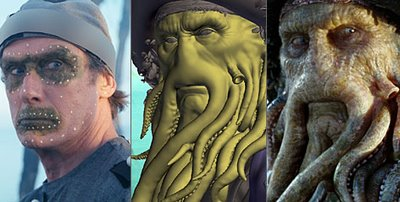
\includegraphics[width=\textwidth]{img/Face-Mocap}
            }
          }
      \pgfputat
          {
            \pgfxy(0,2)}{\pgfbox[left,top]
            {
              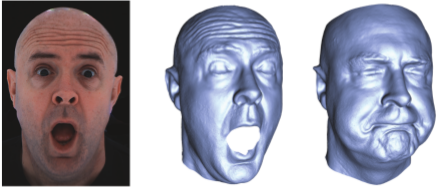
\includegraphics[width=\textwidth]{img/man}
            }
          }

    \end{column}
    
    \begin{column}{0.5\textwidth}
      \pgfputat
          {
            \pgfxy(0,1.5)}{\pgfbox[left,top]
            {
              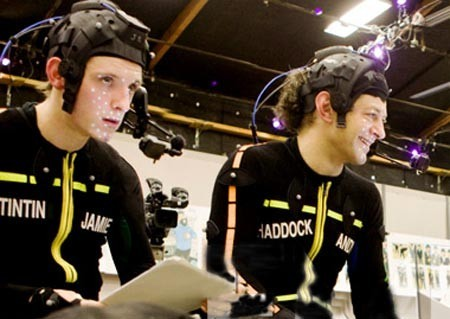
\includegraphics[width=\textwidth]{img/Making-of-Tintin-Spielberg_scaledown_450}
            }
          }
    \end{column}
  \end{columns}
\end{frame}


\section{Projet}
\begin{frame}{Le projet}
  \begin{block}{Objectif}
    \begin{itemize}
    \item Capturer des performances expressives très
      détaillées en utilisant un matériel de prix accessible
    \end{itemize}
  \end{block}

  \begin{bkblock}{Matériel}
    \begin{centering}
      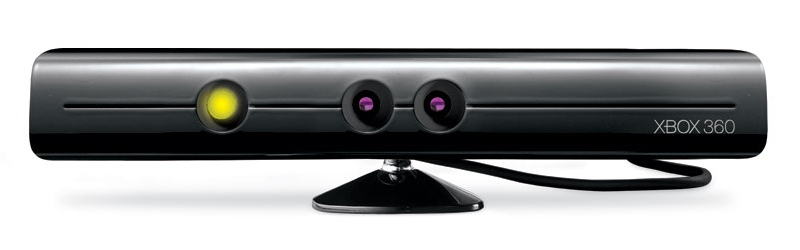
\includegraphics[scale=0.2]{img/kinect}
    \end{centering}
  \end{bkblock}

  \begin{greyblock}{Environement}
    \begin{center}
      
\includegraphics[scale=0.1]{img/linux}
      \hspace{3mm}
      
\includegraphics[scale=0.3]{img/git}
      \hspace{3mm}
      
\includegraphics[scale=0.1]{img/openmp}
      \hspace{3mm}
      
\includegraphics[scale=0.1]{img/qt}
      \hspace{3mm}
      
\includegraphics[scale=0.3]{img/eigen}
    \end{center}
  \end{greyblock}

    
\end{frame}

\begin{frame}{De la capture à la reconstruction finale}
    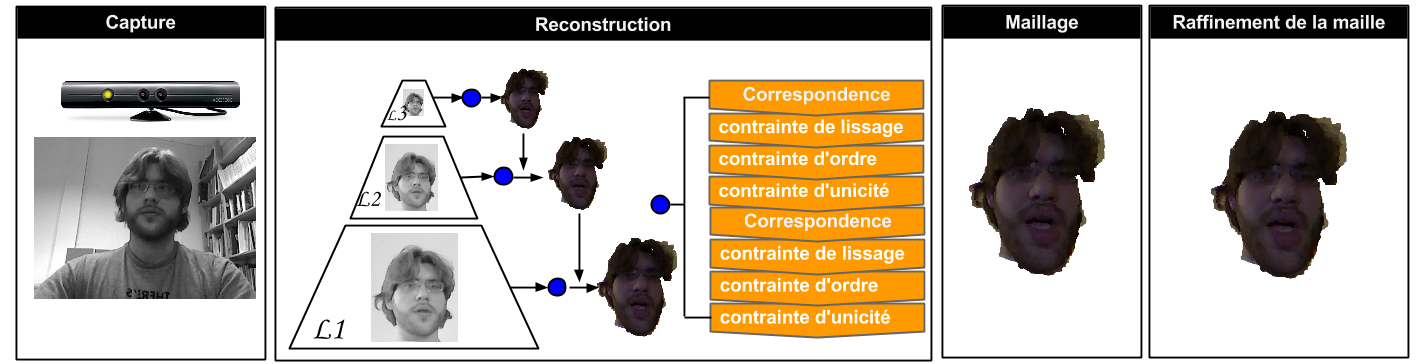
\includegraphics[width=\textwidth]{img/projSystem}
\end{frame}

\begin{frame}{Les étapes}
  \begin{center}
    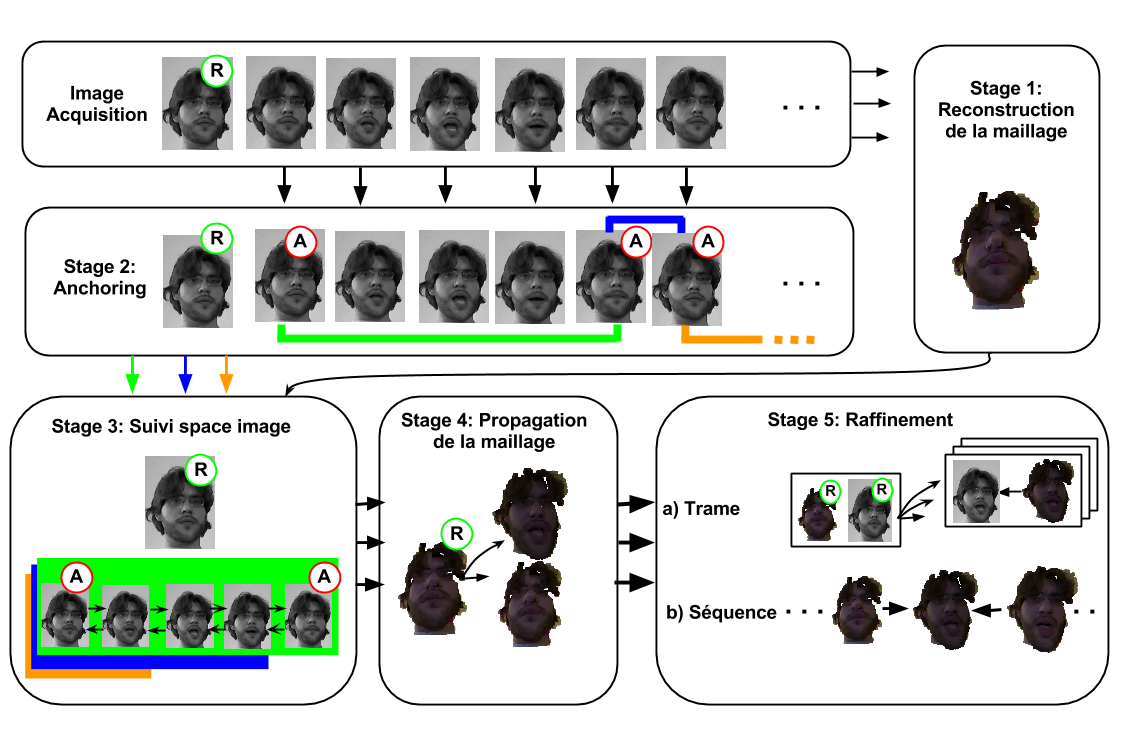
\includegraphics[width=\textwidth]{img/projDiagram}
  \end{center}
\end{frame}


\section{Résultats}
\begin{frame}{}
\end{frame}{}


\section{Conclusion}

\begin{frame}{Conclusion}
  
  \begin{columns}
    \begin{column}{0.5\textwidth}
      
      \begin{beamerboxesrounded}[shadow=true]{Kinect}
        \begin{itemize}
        \item Faible précision
        \item Carte de profondeur incomplète
        \item Adaptation de l'algorithme
        \end{itemize}
      \end{beamerboxesrounded}
    \end{column}    
    
    \begin{column}{0.5\textwidth}
      \begin{beamerboxesrounded}[shadow=true]{Algorithme}

        \begin{itemize}
        \item Résultat bruité 
        \item Interferance de l'illumination
        \end{itemize}

      \end{beamerboxesrounded}

    \end{column}    
  \end{columns}    
  
\end{frame}


\begin{frame}{}
  \begin{figure}
    \begin{centering}
      \Huge Demostration!
      \par\end{centering}
  \end{figure}
\end{frame}

% 
% Questions
% 
\begin{frame}{}
  \begin{figure}
    \begin{centering}
      
\includegraphics[scale=0.1]{img/Icon-round-Question_mark.jpg}
      \par\end{centering}
  \end{figure}
\end{frame}

\end{document}


